{\color{red}\noindent 
Completar frame relay y explicar MPLS
\begin{itemize}
\item Explicar lo que falta de FR
\item Explicar la arquitectura de MPLS
\end{itemize}
}\\

\section*{Frame Relay}
Frame Relay es una tecnología de protocolo de capa de enlace de datos diseñada para conectar redes de área local (LAN) y transferir datos a través de redes de área extensa (WAN). Frame Relay comparte parte de la misma tecnología subyacente que X.25 y alcanzó cierta popularidad en los Estados Unidos como parte de la infraestructura para sistemas de redes digitales de servicios integrados (ISDN) vendidos a clientes comerciales. Se considera el reemplazo de la tecnología de conmutación de paquetes X.25 anterior.
\subsubsection*{Funcionamiento}

Frame Relay admite la multiplexación de tráfico de múltiples conexiones a través de un enlace físico compartido. Utiliza componentes de hardware, incluidos enrutadores de tramas, puentes y conmutadores, para empaquetar datos en mensajes de retransmisión de tramas individuales. Cada conexión utiliza un identificador de conexión de enlace de datos (DLCI) de 10 bits para direccionamiento de canal único. \\{ }\\
Hay dos tipos de conexión. Los circuitos virtuales permanentes (PVC) son para conexiones persistentes que deben mantenerse durante períodos prolongados, incluso si no se transfieren datos de forma activa. Los circuitos virtuales conmutados (SVC) son para conexiones temporales que duran solo una sesión. Frame Relay logra un mejor rendimiento que X.25 a un costo menor al no realizar la corrección de errores. La corrección de errores se pasa  a otros componentes de la red para reducir la latencia de la red. También admite tamaños de paquetes de longitud variable para un uso más eficiente del ancho de banda de la red.\\{ }\\
Frame Relay opera sobre líneas de fibra óptica o ISDN y es compatible con diferentes protocolos de red de nivel superior, incluido el protocolo de Internet (IP).

\begin{center}
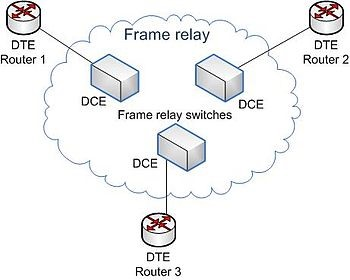
\includegraphics[scale=0.66]{Imagenes/FR.jpg}
\end{center}

\subsection*{Características}
\begin{itemize}
\item Frame Relay es un servicio sin conexión, lo que significa que cada paquete de datos que pasa por la red contiene información de dirección
\item Frame Relay es un servicio que se proporciona con una variedad de velocidades desde 56 Kbs hasta 25 Mbs. 
\item Las tramas son de longitud variable y va hasta 4,096 bytes
\item Opera a alta velocidad (1.544 Mbps a 44.376 Mbps).
\item Opera solo en las capas física y de enlace de datos. Por lo tanto, se puede usar fácilmente en Internet.
\item Frame Relay solo puede detectar errores (en la capa de enlace de datos). Pero no hay control de flujo o control de errores.


\end{itemize}

\section*{MPLS (Multiprotocol Label Switching)}
Multiprotocol Label Switching o MPLS, por su traducción: conmutación de etiquetas multiprotocolo, es un estándar para transmitir datos bajo diferentes etiquetas, creado por la Internet Engineering Task Force, una organización dedicada a mejorar el flujo de trabajo de Internet. Se creó con la finalidad de unificar diversos tipos de datos transmitidos a través de la misma red de para enviar paquetes de información que no generen un problema de velocidad. 
\subsection*{Arquitectura}
Los paquetes se reenvían en una red MPLS basada en etiquetas. los dispositivos de red que intercambian etiquetas MPLS y los paquetes de reenvío son enrutadores de conmutación de etiquetas o label switching routers (LSR), que forman un dominio MPLS. Los LSR que residen en el borde del dominio MPLS y se conectan a otras redes se denominan enrutadores de borde de etiqueta o label edge routers (LER), y los LSR dentro del dominio MPLS son LSR centrales.

\begin{center}
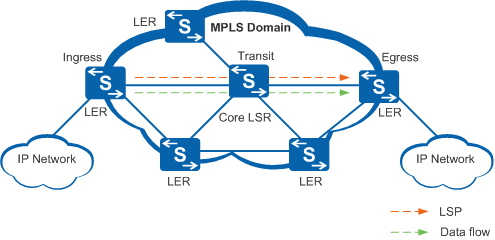
\includegraphics[scale=0.66]{Imagenes/MPLS.png}
\end{center}


\begin{thebibliography}{9}

\bibitem{xx}
What Is Frame Relay Packet-Switching? \href{https://www.lifewire.com/definition-of-frame-relay-817947}{https://www.lifewire.com/definition-of-frame-relay-817947}


\bibitem{xx2}

Conociendo la arquitectura básica de una red MPLS \href{https://forum.huawei.com/enterprise/es/conociendo-la-arquitectura-b\%C3\%A1sica-de-una-red-mpls/thread/582304-100237}{https://forum.huawei.com/enterprise/es/conociendo-la-arquitectura-b\%C3\%A1sica-de-una-red-mpls/thread/582304-100237}

\bibitem{xx3}
Frame Relay \href{https://ccnadesdecero.es/frame-relay/}{https://ccnadesdecero.es/frame-relay/}

\bibitem{xx4}
Elementos de una red MPLS \href{https://www.ramonmillan.com/tutoriales/mpls.php{\#}elementosredmpls}{https://www.ramonmillan.com/tutoriales/mpls.php{\#}elementosredmpls}

\bibitem{xx5}
MPLS Architecture \href{ https://www.mplsinfo.org/architecture.html}{ https://www.mplsinfo.org/architecture.html}

\end{thebibliography}

